\chapter{Limiti Inferiori per l'Ordinamento, Quicksort Dual-Pivot e Bounded Quicksort}
\label{cha:lecture-four}

\begin{center}
  \textbf{Lezione 4}\\
  \emph{Limiti Inferiori (RAM vs Modello a Due Livelli), Quicksort Dual-Pivot e Bounded Quicksort}\\[0.5em]
  Data: 28 Settembre 2026
\end{center}

In questo capitolo viene affrontata l'analisi teorica e ingegneristica dei limiti inferiori di complessità per il problema fondamentale dell'ordinamento basato su confronti, confrontando il modello RAM classico con il modello a due livelli di Aggarwal e Vitter. Successivamente, l'indagine si sposta sulle moderne evoluzioni architetturali dell'algoritmo \textit{Quicksort}: viene analizzato il problema dei valori duplicati e l'algoritmo \textit{Dual-Pivot Quicksort} introdotto da Yaroslavskiy, per poi esaminare formalmente la variante \textit{Bounded Quicksort} (BQS), dimostrando come l'eliminazione della ricorsione in coda (\textit{tail recursion elimination}) e il partizionamento controllato garantiscano uno spazio ausiliario rigorosamente limitato a $\Theta(\log_2 n)$ unito alla massima efficienza di cache tramite cutoff a \textit{Insertion Sort}.

\FloatBarrier
\section{Modello RAM: Limiti Inferiori e Alberi di Decisione}
\label{sec:ram-lower-bounds}

Nel modello di calcolo RAM (\textit{Random Access Machine}) standard, un algoritmo basato su confronti (\textit{comparison-based algorithm}) non può accedere alla rappresentazione binaria interna delle chiavi per estrarne cifre o bit (come invece avviene negli algoritmi di tipo \textit{Radix Sort}), ma può acquisire informazioni sull'ordine reciproco degli elementi esclusivamente attraverso confronti binari del tipo:
\begin{equation}
  A < B, \quad A = B, \quad \text{oppure} \quad A > B.
\end{equation}
Assumendo, senza perdita di generalità per l'analisi del limite inferiore, che tutte le chiavi in ingresso siano reciprocamente distinte, ogni confronto elementare ammette un esito strettamente dicotomico ($<$ oppure $>$).

\subsection{Il Modello dell'Albero di Decisione}
\label{subsec:decision-tree-model}

La classe degli algoritmi deterministici basati su confronti viene formalmente modellata mediante la struttura astratta dell'\textbf{Albero di Decisione} (\textit{Decision Tree}):

\begin{itemize}
  \item \textbf{Nodi interni:} Ciascun nodo interno rappresenta un singolo confronto elementare tra una coppia di elementi o posizioni dell'input, denotato convenzionalmente con $[A : B]$. Poiché le chiavi sono distinte, dal nodo si dipartono esattamente due archi uscenti, corrispondenti agli esiti possibili: l'arco sinistro associato all'evento $A < B$ e l'arco destro associato all'evento $A > B$. L'albero risulta pertanto un albero binario proprio.
  \item \textbf{Cammino radice-foglia:} Per ogni specifica istanza di input di dimensione $n$, l'algoritmo deterministico segue un unico cammino orientato discendente dalla radice verso una foglia. Ciascun nodo visitato lungo il cammino corrisponde a un confronto eseguito; la lunghezza del cammino (numero di archi attraversati) riflette il numero di confronti effettuati per quella specifica configurazione. La lunghezza del cammino più lungo dalla radice a una foglia coincide con l'\textbf{altezza} $t$ dell'albero di decisione e quantifica il tempo di esecuzione nel caso peggiore $T(n)$.
  \item \textbf{Foglie:} Ciascuna foglia corrisponde alla terminazione del processo di calcolo e racchiude la risposta o configurazione risolutiva finale del problema (ad esempio, la corretta permutazione degli indici che ordina l'array, o l'indice in cui risiede la chiave cercata).
\end{itemize}

In \autoref{fig:decision-tree-model} viene illustrata la topologia generale di un albero di decisione binario per un generico problema basato su confronti.

\begin{figure}[H]
  \centering
  \begin{tikzpicture}[
    scale=0.92,
    node distance=1.5cm,
    cmp/.style={rectangle, draw=blue!75!black, fill=blue!8, thick, rounded corners=3pt, minimum width=1.9cm, minimum height=0.65cm, font=\small\bfseries, align=center},
    leaf/.style={rectangle, draw=green!60!black, fill=green!12, thick, rounded corners=3pt, minimum width=1.0cm, minimum height=0.62cm, font=\small\bfseries, align=center},
    edgeLbl/.style={font=\scriptsize\bfseries, fill=white, inner sep=1.5pt},
    arr/.style={-{Stealth[scale=1.0]}, thick, draw=blue!80!black}
  ]
    % Radice
    \node[cmp] (root) at (0, 0) {$A : B$};
    
    % Livello 1
    \node[cmp] (L1) at (-2.8, -1.4) {$C : D$};
    \node[cmp] (R1) at (2.8, -1.4) {$E : F$};
    
    \draw[arr] (root) -- node[edgeLbl, above left] {$A < B$} (L1);
    \draw[arr] (root) -- node[edgeLbl, above right] {$A > B$} (R1);
    
    % Livello 2
    \node[cmp] (LL2) at (-4.4, -2.8) {$G : H$};
    \node[cmp] (LR2) at (-1.6, -2.8) {$I : J$};
    \node[cmp] (RL2) at (1.6, -2.8) {$K : L$};
    \node[cmp] (RR2) at (4.4, -2.8) {$M : N$};
    
    \draw[arr] (L1) -- node[edgeLbl, left] {$<$} (LL2);
    \draw[arr] (L1) -- node[edgeLbl, right] {$>$} (LR2);
    \draw[arr] (R1) -- node[edgeLbl, left] {$<$} (RL2);
    \draw[arr] (R1) -- node[edgeLbl, right] {$>$} (RR2);
    
    % Punti di sospensione per profondità intermedia
    \node at (-4.4, -3.6) {$\vdots$};
    \node at (-1.6, -3.6) {$\vdots$};
    \node at (1.6, -3.6) {$\vdots$};
    \node at (4.4, -3.6) {$\vdots$};
    
    % Foglie terminali distinte (soluzioni del problema)
    \node[leaf] (leaf1) at (-5.1, -4.7) {$S_1$};
    \node[leaf] (leaf2) at (-3.7, -4.7) {$S_2$};
    \node[leaf] (leaf3) at (-1.6, -4.7) {$S_3$};
    \node[font=\small\bfseries, text=gray!80!black] (leafmid1) at (0.0, -4.7) {$\dots$};
    \node[leaf] (leafk) at (1.6, -4.7) {$S_k$};
    \node[font=\small\bfseries, text=gray!80!black] (leafmid2) at (2.65, -4.7) {$\dots$};
    \node[leaf] (leafn1) at (3.7, -4.7) {$S_{n-1}$};
    \node[leaf] (leafn) at (5.1, -4.7) {$S(n)$};
    
    \draw[arr, dashed] (-4.4, -3.9) -- (leaf1);
    \draw[arr, dashed] (-4.4, -3.9) -- (leaf2);
    \draw[arr, dashed] (-1.6, -3.9) -- (leaf3);
    \draw[arr, dashed] (1.6, -3.9) -- (leafk);
    \draw[arr, dashed] (4.4, -3.9) -- (leafn1);
    \draw[arr, dashed] (4.4, -3.9) -- (leafn);
    
    % Quota dell'altezza t
    \draw[{Stealth[scale=1.1]}-{Stealth[scale=1.1]}, thick, draw=red!70!black] (6.0, 0) -- (6.0, -4.7) 
      node[midway, right=4pt, align=left, font=\footnotesize\bfseries, text=red!80!black] {Altezza $t$\\ $\ge \log_2 S(n)$};
    \draw[draw=gray!50, dashed] (root.east) -- (6.1, 0);
    \draw[draw=gray!50, dashed] (leafn.east) -- (6.1, -4.7);
    
    % Graffa inferiore per numero di foglie
    \draw[decorate, decoration={brace, amplitude=6pt, mirror}, thick, draw=green!60!black] (-5.7, -5.2) -- (5.7, -5.2)
      node[midway, below=7pt, font=\small\bfseries, text=green!50!black] {Foglie (soluzioni distinte): numero totale $\le 2^t$, con $2^t \ge S(n)$};
  \end{tikzpicture}
  \caption{Modello dell'albero di decisione binario per algoritmi basati su confronti. I nodi interni rappresentano i confronti elementari; le foglie rappresentano le soluzioni distinte ammissibili ($S_1, S_2, \dots, S(n)$). Il cammino più lungo determina il tempo nel caso peggiore.}
  \label{fig:decision-tree-model}
\end{figure}

\subsection{Il Teorema Generale dell'Informazione}
\label{subsec:general-information-theorem}

Il legame tra il numero di soluzioni distinte di un problema e il numero minimo di confronti necessari a risolverlo è sancito dal seguente teorema fondamentale della teoria dell'informazione applicata agli algoritmi.

\begin{theorem}[Teorema Generale dell'Informazione per Alberi di Decisione]
\label{thm:information-theoretic-bound}
Sia $P$ un problema computazionale risolvibile tramite un algoritmo deterministico basato su confronti. Se per un input di dimensione $n$ il problema ammette $S(n)$ soluzioni distinte (ciascuna delle quali deve poter essere restituita dall'algoritmo per opportune istanze dell'input), allora qualsiasi algoritmo deterministico basato su confronti richiede nel caso peggiore un tempo:
\begin{equation}
  T(n) = \Omega(\log_2 S(n)).
\end{equation}
\end{theorem}

\begin{proof}
Consideriamo l'albero di decisione binario associato a un qualsiasi algoritmo deterministico corretto per il problema $P$. Sia $t$ l'altezza dell'albero, ovvero la lunghezza massima di un cammino dalla radice a una foglia.

Poiché a ogni passo il confronto è binario (avendo assunto chiavi distinte), ogni nodo interno possiede al più $2$ figli. Per induzione sull'altezza, un albero binario di altezza $t$ possiede al massimo un numero di foglie $L$ pari a:
\begin{equation}
  L \le 2^t.
\end{equation}
Affinché l'algoritmo sia corretto su qualsiasi istanza ammissibile, l'albero di decisione deve essere in grado di produrre ciascuna delle $S(n)$ possibili risposte distinte. Ne consegue che ogni soluzione distinta deve essere associata ad almeno una foglia distinta dell'albero (se due soluzioni distinte convergessero sulla medesima foglia, l'algoritmo fallirebbe nel distinguerle, restituendo un risultato errato per almeno una delle istanze corrispondenti). Pertanto, deve necessariamente valere la disuguaglianza:
\begin{equation}
  2^t \ge L \ge S(n).
\end{equation}
Applicando la funzione logaritmica in base $2$ (strettamente monotona crescente) ad ambo i membri, si ottiene:
\begin{equation}
  t \ge \log_2 S(n).
\end{equation}
Poiché il tempo di esecuzione nel caso peggiore $T(n)$ coincide per definizione con l'altezza $t$ dell'albero, si conclude che:
\begin{equation}
  T(n) \ge \log_2 S(n) \implies T(n) = \Omega(\log_2 S(n)).
\end{equation}
\end{proof}

\subsection{Applicazioni Fondamentali: Ricerca e Ordinamento}
\label{subsec:search-and-sort-applications}

Il \autoref{thm:information-theoretic-bound} consente di ricavare immediatamente i limiti inferiori canonici per due problemi cardine della computazione in memoria interna:

\begin{enumerate}
  \item \textbf{Ricerca di una chiave (\textit{Searching}):}
  Dato un array ordinato di $n$ elementi e una chiave cercata $K$, l'algoritmo deve stabilire se $K$ è presente nell'array e, in caso affermativo, restituire l'indice $i \in \{1, 2, \dots, n\}$ corrispondente; se la chiave è assente, restituisce un simbolo speciale di fallimento $\bot$. L'insieme delle possibili risposte distinte è dunque:
  \begin{equation}
    S(n) = \{1, 2, \dots, n\} \cup \{\bot\} \implies |S(n)| = n + 1.
  \end{equation}
  Applicando il teorema:
  \begin{equation}
    T_{\text{Search}}(n) \ge \log_2(n + 1) = \Omega(\log_2 n).
  \end{equation}
  Questo limite inferiore attesta l'ottimalità asintotica della \textit{Ricerca Binaria} (\textit{Binary Search}), la quale opera esattamente in $\Theta(\log_2 n)$ confronti.

  \item \textbf{Ordinamento (\textit{Sorting}):}
  Dato un vettore di $n$ elementi distinti, ordinare l'array equivale a identificare quale tra tutte le possibili permutazioni degli indici sia quella che dispone le chiavi in ordine non decrescente. Poiché l'insieme $\{1, 2, \dots, n\}$ ammette esattamente $n!$ permutazioni distinte, il numero di soluzioni possibili corrisponde a:
  \begin{equation}
    S(n) = n!.
  \end{equation}
  Applicando il teorema dei limiti inferiori:
  \begin{equation}
    T_{\text{Sort}}(n) \ge \log_2(n!).
  \end{equation}
  Per esprimere questo valore in forma asintotica esplicita, ricorriamo all'\textbf{approssimazione di Stirling} per il fattoriale:
  \begin{equation}
    n! \approx \sqrt{2\pi n} \left(\frac{n}{e}\right)^n \implies \ln(n!) = n \ln n - n + \mathcal{O}(\ln n).
  \end{equation}
  Convertendo il logaritmo in base $2$:
  \begin{equation}
    \log_2(n!) = n \log_2 n - n \log_2 e + \Theta(\log_2 n) = \Theta(n \log_2 n).
  \end{equation}
  Alternativamente, mediante una limitazione inferiore elementare per metà dei termini:
  \begin{align}
    n! &\ge \prod_{i = \lceil n/2 \rceil}^{n} i \ge \left(\frac{n}{2}\right)^{n/2}, \\
    \log_2(n!) &\ge \frac{n}{2} \log_2\left(\frac{n}{2}\right) = \frac{n}{2}(\log_2 n - 1) = \Omega(n \log_2 n).
  \end{align}
  Si conclude che:
  \begin{equation}
    T_{\text{Sort}}(n) = \Omega(n \log_2 n).
  \end{equation}
  Qualsiasi algoritmo deterministico o randomizzato basato su confronti (come \textit{Merge Sort}, \textit{Heap Sort} o il tempo atteso di \textit{Quicksort}) non può scendere al di sotto della soglia asintotica $\Omega(n \log_2 n)$ nel modello RAM.
\end{enumerate}

\FloatBarrier
\section{Modello a Due Livelli: Limite Inferiore di Aggarwal-Vitter}
\label{sec:aggarwal-vitter-lower-bound}

Nel modello di memoria a due livelli di Aggarwal e Vitter~\cite{aggarwal1988}, il costo di esecuzione non è misurato dai confronti elementari della CPU, bensì dal numero $t$ di operazioni di I/O, ciascuna delle quali trasferisce un intero blocco di dimensione $B$ tra il disco non volatile e la memoria interna (RAM) di capacità pari a $M$ elementi.

\subsection{La Natura dell'I/O e i Confronti Gratuiti in Memoria Interna}
\label{subsec:free-comparisons-intuition}

L'analisi tradizionale dell'albero di decisione binario non è direttamente applicabile al calcolo degli I/O:
\begin{itemize}
  \item Una singola operazione di lettura dal disco carica contemporaneamente $B$ elementi in memoria rapida.
  \item Una volta che questi $B$ elementi risiedono nella RAM accanto agli altri $M - B$ elementi già presenti, la CPU può eseguire \textbf{un numero arbitrariamente elevato di confronti interni a costo zero di I/O}.
  \item Tali confronti interni "gratuiti" consentono di riordinare istantaneamente tutti gli $M$ elementi residenti in RAM, restringendo drasticamente il ventaglio delle permutazioni globali ancora compatibili con lo stato dei dati.
\end{itemize}

Pertanto, per determinare il lower bound su memoria esterna, è necessario costruire un \textbf{Albero di Decisione di I/O}, in cui ogni nodo rappresenta un'operazione di I/O (lettura di un blocco di taglia $B$) e gli archi uscenti corrispondono a tutte le possibili sistemazioni informative derivanti dall'interazione tra i $B$ elementi letti e gli $M - B$ elementi già presenti in memoria interna.

\subsection{Calcolo del Grado di Diramazione (Fan-out) dell'Albero di I/O}
\label{subsec:fanout-calculation}

Quando un blocco di $B$ elementi viene trasferito dal disco alla memoria interna (che accoglie $M$ elementi totali, di cui $M - B$ preesistenti e $B$ appena caricati), distinguiamo due scenari operativi:

\begin{enumerate}
  \item \textbf{Lettura di un "Nuovo Blocco" (\textit{New Block}):}
  Il blocco viene letto dal disco per la primissima volta: gli elementi in esso contenuti non sono mai stati osservati in precedenza da alcun'altra operazione dell'algoritmo.
  \begin{itemize}
    \item L'ordine reciproco dei $B$ elementi è totalmente ignoto: essi possono presentarsi internamente in una qualsiasi delle $B!$ permutazioni relative possibili.
    \item Una volta caricati in RAM, i $B$ nuovi elementi devono essere posizionati reciprocamente rispetto agli $M - B$ elementi già residenti, determinando quale sia la loro collocazione ordinata comune nell'insieme totale di $M$ elementi. Il numero di modi in cui $B$ elementi indistinguibili nella loro posizione possono intercalarsi tra gli $M$ slot totali è dato dal coefficiente binomiale:
    \begin{equation}
      \binom{M}{B} = \frac{M!}{B! \, (M - B)!}.
    \end{equation}
  \end{itemize}
  Moltiplicando le $B!$ configurazioni d'ordine interno per i $\binom{M}{B}$ modi di intercalamento, il fattore di diramazione (\textit{fan-out}) $X$ generato dalla lettura di un nuovo blocco risulta:
  \begin{equation}
    X = (B!) \cdot \binom{M}{B}.
    \label{eq:fanout-new-block}
  \end{equation}

  \item \textbf{Rilettura di un "Vecchio Blocco" (\textit{Old Block}):}
  Il blocco era già stato caricato, ordinato internamente e successivamente scritto su disco in una fase precedente della computazione (si pensi a un run generato durante un passo di merge).
  \begin{itemize}
    \item L'ordine relativo interno dei suoi $B$ elementi è già integralmente noto alla computazione; non si ottiene pertanto alcuna nuova informazione sul loro ordine intrinseco (fattore $1$ al posto di $B!$).
    \item L'unico incremento informativo risiede nell'intercalamento dei $B$ elementi con gli altri $M - B$ elementi attualmente residenti in memoria interna.
  \end{itemize}
  Il fattore di diramazione (\textit{fan-out}) $Y$ per la rilettura di un vecchio blocco è quindi:
  \begin{equation}
    Y = \binom{M}{B}.
    \label{eq:fanout-old-block}
  \end{equation}
\end{enumerate}

In \autoref{fig:io-decision-tree} viene schematizzata la biforcazione logica e la cardinalità delle diramazioni per le due tipologie di trasferimento I/O.

\begin{figure}[H]
  \centering
  \begin{tikzpicture}[
    scale=0.95,
    box/.style={rectangle, draw=blue!80!black, fill=blue!8, thick, rounded corners=4pt, minimum width=4.2cm, minimum height=1.0cm, align=center, font=\small\bfseries},
    branch/.style={rectangle, draw=orange!80!black, fill=orange!8, thick, rounded corners=3pt, minimum width=5.5cm, minimum height=2.2cm, align=left, font=\footnotesize},
    arr/.style={-{Stealth[scale=1.1]}, thick, draw=blue!70!black}
  ]
    % Nodo I/O superiore
    \node[box] (ioNode) at (0, 2.7) {Operazione di Lettura I/O\\(Carica $B$ elementi in memoria $M$)};
    
    % Ramo Sinistro: Nuovo Blocco
    \node[branch] (newBlock) at (-3.8, -0.8) {
      \textbf{\textcolor{orange!90!black}{A) Nuovo Blocco (\textit{New Block})}}\\[3pt]
      $\bullet$ $B$ elementi mai osservati prima;\\
      $\bullet$ $B!$ permutazioni interne possibili;\\
      $\bullet$ $\binom{M}{B}$ modi di intercalarsi tra gli $M$ slot;\\[4pt]
      \textbf{Grado di diramazione (Fan-out):}\\[2pt]
      \null\hfill $X = (B!) \cdot \binom{M}{B}$\hfill\null
    };
    
    % Ramo Destro: Vecchio Blocco
    \node[branch] (oldBlock) at (3.8, -0.8) {
      \textbf{\textcolor{orange!90!black}{B) Vecchio Blocco (\textit{Old Block})}}\\[3pt]
      $\bullet$ Blocco già processato in precedenza;\\
      $\bullet$ Ordine interno tra i $B$ elementi già noto;\\
      $\bullet$ $\binom{M}{B}$ modi di intercalarsi tra gli $M$ slot;\\[4pt]
      \textbf{Grado di diramazione (Fan-out):}\\[2pt]
      \null\hfill $Y = \binom{M}{B}$\hfill\null
    };
    
    \draw[arr] (ioNode.south) -- ++(0, -0.5) -| node[pos=0.25, above=2pt, font=\scriptsize\bfseries] {Prima lettura} (newBlock.north);
    \draw[arr] (ioNode.south) -- ++(0, -0.5) -| node[pos=0.25, above=2pt, font=\scriptsize\bfseries] {Rilettura successiva} (oldBlock.north);
  \end{tikzpicture}
  \caption{Fattori di diramazione (\textit{fan-out}) nell'albero di decisione di I/O nel modello a due livelli: la lettura di un nuovo blocco apporta informazione d'ordine interno ($B!$) e di intercalamento ($\binom{M}{B}$); la rilettura di un vecchio blocco apporta esclusivamente informazione di intercalamento.}
  \label{fig:io-decision-tree}
\end{figure}

\subsection{Derivazione Formale del Lower Bound di Aggarwal-Vitter}
\label{subsec:formal-derivation-av}

Sia dato un file di ingresso composto da $n$ elementi distinti suddivisi in $N = \frac{n}{B}$ blocchi su disco. Per poter ordinare il file, qualsiasi algoritmo corretto deve necessariamente ispezionare ciascun elemento almeno una volta: ne discende che l'algoritmo deve compiere almeno $\frac{n}{B}$ operazioni di lettura di tipo "Nuovo Blocco".

Se l'algoritmo esegue complessivamente $t$ operazioni di I/O nel caso peggiore, allora:
\begin{itemize}
  \item Esattamente $\frac{n}{B}$ operazioni saranno di tipo "Nuovo Blocco", ciascuna con fattore di diramazione al più $X$.
  \item Le rimanenti $t - \frac{n}{B}$ operazioni saranno (al più) di tipo "Vecchio Blocco", ciascuna con fattore di diramazione al più $Y$.
\end{itemize}

Il numero totale di foglie dell'albero di decisione di I/O rappresenta il numero massimo di permutazioni globali distinguibili dalla sequenza di trasferimenti. Affinché l'algoritmo sia in grado di ordinare correttamente qualsiasi istanza, tale numero di foglie deve risultare almeno pari al numero totale di permutazioni ammissibili $n!$:
\begin{equation}
  X^{\frac{n}{B}} \cdot Y^{\left(t - \frac{n}{B}\right)} \ge n!.
  \label{eq:io-tree-leaves-inequality}
\end{equation}

Sostituendo le espressioni di $X$ ed $Y$ definite nelle equazioni~(\ref{eq:fanout-new-block}) e~(\ref{eq:fanout-old-block}):
\begin{equation}
  \left[ (B!) \cdot \binom{M}{B} \right]^{\frac{n}{B}} \cdot \left[ \binom{M}{B} \right]^{t - \frac{n}{B}} \ge n!.
\end{equation}
Raccogliendo le potenze relative alla base comune $\binom{M}{B}$:
\begin{equation}
  (B!)^{\frac{n}{B}} \cdot \binom{M}{B}^{\frac{n}{B}} \cdot \binom{M}{B}^{t - \frac{n}{B}} \ge n! \implies (B!)^{\frac{n}{B}} \cdot \binom{M}{B}^t \ge n!.
  \label{eq:leaves-compact-inequality}
\end{equation}

Applichiamo il logaritmo in base $2$ a entrambi i membri della disuguaglianza~(\ref{eq:leaves-compact-inequality}):
\begin{equation}
  \log_2\left((B!)^{\frac{n}{B}}\right) + \log_2\left(\binom{M}{B}^t\right) \ge \log_2(n!),
\end{equation}
da cui:
\begin{equation}
  \frac{n}{B} \log_2(B!) + t \log_2\binom{M}{B} \ge \log_2(n!).
  \label{eq:log-leaves-inequality}
\end{equation}

Per sviluppare i termini logaritmici utilizziamo le consuete approssimazioni asintotiche per il fattoriale e per il coefficiente binomiale:
\begin{itemize}
  \item Per l'approssimazione di Stirling: $\log_2(a!) \approx a \log_2 a - a \log_2 e \approx a \log_2 a$.
  \item Per il coefficiente binomiale, ricordando che $\binom{a}{b} \le \left(\frac{e \cdot a}{b}\right)^b$:
  \begin{equation}
    \log_2 \binom{M}{B} \approx B \log_2\left(\frac{M}{B}\right) + \mathcal{O}(B).
  \end{equation}
\end{itemize}

Sostituendo queste espressioni nell'equazione~(\ref{eq:log-leaves-inequality}):
\begin{equation}
  \frac{n}{B} \cdot \left(B \log_2 B\right) + t \cdot \left(B \log_2 \frac{M}{B}\right) \ge n \log_2 n.
\end{equation}
Semplificando il fattore $B$ nel primo termine:
\begin{equation}
  n \log_2 B + t \cdot B \log_2\left(\frac{M}{B}\right) \ge n \log_2 n.
\end{equation}

Isoliamo il termine contenente l'incognita $t$:
\begin{equation}
  t \cdot B \log_2\left(\frac{M}{B}\right) \ge n \log_2 n - n \log_2 B = n \left(\log_2 n - \log_2 B\right) = n \log_2\left(\frac{n}{B}\right).
\end{equation}
Dividendo ambo i membri per la quantità strettamente positiva $B \log_2\left(\frac{M}{B}\right)$:
\begin{equation}
  t \ge \frac{n \log_2\left(\frac{n}{B}\right)}{B \log_2\left(\frac{M}{B}\right)} = \frac{n}{B} \cdot \frac{\log_2(n / B)}{\log_2(M / B)}.
\end{equation}

Ricorrendo alla proprietà del cambio di base dei logaritmi ($\frac{\log_2 a}{\log_2 b} = \log_b a$), otteniamo formalmente il celebre teorema di Aggarwal e Vitter.

\begin{theorem}[Limite Inferiore di Aggarwal-Vitter per l'Ordinamento]
\label{thm:aggarwal-vitter-bound}
Nel modello di memoria a due livelli, qualsiasi algoritmo deterministico o randomizzato basato su confronti richiede nel caso peggiore un numero di trasferimenti I/O pari a:
\begin{equation}
  \text{I/O}_{\text{Sort}}(n) = \Omega\left(\frac{n}{B} \log_{M/B}\left(\frac{n}{B}\right)\right) = \Omega\left(\frac{n}{B} \frac{\log(n / B)}{\log(M / B)}\right).
\end{equation}
\end{theorem}

\begin{property}[Ottimalità Asintotica del Multiway Merge Sort]
Il limite inferiore di Aggarwal e Vitter dimostra che il \textbf{Multiway Merge Sort} ($k$-Way Merge Sort con fattore di merge $k = \frac{M}{B} - 1$) analizzato nella Lezione~\ref{cha:lecture-three} (\autoref{sec:multiway-merge-sort}) è \textbf{asintoticamente ottimo}: il numero di I/O spesi per ordinare l'array coincide esattamente con la barriera teorica insuperabile imposta dalla teoria dell'informazione su memoria esterna.
\end{property}

\FloatBarrier
\section{Quicksort: Gestione dei Duplicati e Dual-Pivot Quicksort}
\label{sec:quicksort-and-dual-pivot}

\textit{Quicksort} è un algoritmo basato sul paradigma \textit{Divide et Impera} di tipo distributivo (\textit{distribution-based}): anziché dividere rigidamente l'array per posizione (come in \textit{Merge Sort}) per poi unire i risultati ordinati, Quicksort partiziona i dati in base al valore di una o più chiavi privilegiate denominate \textbf{pivot}, delegando l'intero lavoro di ordinamento alla fase di distribuzione (\textit{partition}).

\subsection{Il Problema dei Valori Uguali (Equal Values)}
\label{subsec:equal-values-problem}

Nelle implementazioni didattiche standard di Quicksort basate sul partizionamento a due vie (\textit{2-way partitioning}, schema di Lomuto o di Hoare):
\begin{itemize}
  \item L'array viene ripartito in due sole categorie: elementi $\le p$ da una parte ed elementi $> p$ dall'altra.
  \item Qualora l'array contenga una frequenza elevata di elementi identici al pivot $p$ (nel caso limite, un array composto esclusivamente da elementi tutti uguali, $S[i] = c, \forall i$), tale schema inserisce tutti gli elementi duplicati all'interno della medesima partizione.
  \item La dimensione della sotto-istanza si riduce di una sola unità a ogni invocazione ($1$ contro $n-1$), degradando l'albero di ricorsione a un albero degenere di altezza $\Theta(n)$ e il tempo complessivo di calcolo alla complessità pessima:
  \begin{equation}
    T(n) = T(n - 1) + \Theta(n) = \Theta(n^2).
  \end{equation}
\end{itemize}

\begin{definition}[Partizionamento a Tre Vie (Dutch National Flag)]
La soluzione classica al problema dei duplicati, formulata da Edsger Dijkstra~\cite{dijkstra1976} con il problema della bandiera olandese, consiste nel partizionare l'array in \textbf{tre zone contigue}:
\begin{equation}
  [\, < p \quad \mid \quad = p \quad \mid \quad > p \,].
\end{equation}
Gli elementi strettamente uguali al pivot ($= p$) si trovano già nella loro collocazione definitiva e vengono \textbf{esclusi dalle successive chiamate ricorsive}, le quali vengono lanciate esclusivamente sulle fasce $[< p]$ e $[> p]$. Su array con elementi tutti uguali, l'algoritmo converge in tempo strettamente lineare $\mathcal{O}(n)$.
\end{definition}

\subsection{Algoritmo di Partizionamento a 3 Vie ed Esempio Esecutivo}
\label{subsec:3way-quicksort-example}

Per implementare concretamente il partizionamento a tre vie (\textit{Dutch National Flag}) in Quicksort, si adotta comunemente lo schema lineare ideato da Dijkstra e formalizzato da Sedgewick~\cite{sedgewick1978}. 

Dato un sotto-array $S[\text{lo} \dots \text{hi}]$ e scelto come pivot l'elemento iniziale $p = S[\text{lo}]$, l'algoritmo mantiene tre indici operativi durante la scansione:
\begin{itemize}
  \item \textbf{Puntatore $lt$ (\textit{less than}):} delimita a sinistra gli elementi strettamente inferiori al pivot. L'invariante garantisce che $S[k] < p$ per ogni $\text{lo} \le k < lt$. Inizialmente $lt = \text{lo}$.
  \item \textbf{Puntatore $i$ (cursore di scansione):} scorre gli elementi dell'array. L'invariante assicura che $S[k] = p$ per ogni $lt \le k < i$. Inizialmente $i = \text{lo} + 1$.
  \item \textbf{Puntatore $gt$ (\textit{greater than}):} delimita a destra gli elementi strettamente superiori al pivot. L'invariante garantisce che $S[k] > p$ per ogni $gt < k \le \text{hi}$. Inizialmente $gt = \text{hi}$.
  \item L'intervallo $S[i \dots gt]$ contiene gli elementi ancora non esaminati.
\end{itemize}

A ogni iterazione, finché $i \le gt$, si confronta l'elemento corrente $S[i]$ con il pivot $p$:
\begin{enumerate}
  \item \textbf{Se $S[i] < p$:} si scambia $S[lt]$ con $S[i]$, quindi si incrementano entrambi gli indici ($lt \leftarrow lt + 1$, $i \leftarrow i + 1$). Poiché per invariante la cella $S[lt]$ conteneva un elemento $= p$, lo scambio sposta il valore minore a sinistra e posiziona un duplicato del pivot in $S[i]$, consentendo a $i$ di avanzare.
  \item \textbf{Se $S[i] > p$:} si scambia $S[i]$ con $S[gt]$, quindi si decrementa solo $gt$ ($gt \leftarrow gt - 1$). L'indice $i$ \textbf{non avanza}, poiché l'elemento appena scambiato da $S[gt]$ non è ancora stato esaminato.
  \item \textbf{Se $S[i] == p$:} l'elemento si trova già nella collocazione centrale corretta; si incrementa unicamente il cursore di scansione ($i \leftarrow i + 1$).
\end{enumerate}

Al termine della procedura ($i > gt$), l'array risulta ripartito nelle tre zone: $S[\text{lo} \dots lt-1] < p$, $S[lt \dots gt] = p$ e $S[gt+1 \dots \text{hi}] > p$. Le successive chiamate ricorsive vengono invocate \textbf{esclusivamente} su $S[\text{lo} \dots lt-1]$ e su $S[gt+1 \dots \text{hi}]$, escludendo l'intero blocco di duplicati. Le proprietà formali di conservazione dimensionale di tali partizioni e l'integrazione con la selezione rapida (\textit{Quickselect}) e la ricorrenza del tempo atteso vengono approfondite nella Lezione~\ref{cha:lecture-five} (\autoref{sec:3way-partitioning}).

In \autoref{tab:3way-execution-trace} viene riportata l'evoluzione dettagliata passo per passo dei tre puntatori e del contenuto dell'array durante l'esecuzione dell'algoritmo con pivot $p = 4$.

\begin{table}[H]
  \centering
  \small
  \begin{tabularx}{\textwidth}{c c c c >{\centering\arraybackslash}p{2.6cm} >{\raggedright\arraybackslash}X >{\centering\arraybackslash}p{3.2cm}}
    \toprule
    \textbf{Passo} & $\boldsymbol{i}$ & $\boldsymbol{lt}$ & $\boldsymbol{gt}$ & \textbf{Confronto} & \textbf{Azione} & \textbf{Stato Array} \\
    \midrule
    Init & 1 & 0 & 7 & Pivot $p = 4$ & Inizializzazione & $[4, 7, 2, 4, 1, 4, 8, 3]$ \\
    1 & 1 & 0 & 7 & $S[1]=7 > 4$ & $\text{SWAP}(S[1], S[7])$, $gt \leftarrow 6$ & $[4, 3, 2, 4, 1, 4, 8, 7]$ \\
    2 & 1 & 0 & 6 & $S[1]=3 < 4$ & $\text{SWAP}(S[0], S[1])$, $lt \leftarrow 1$, $i \leftarrow 2$ & $[3, 4, 2, 4, 1, 4, 8, 7]$ \\
    3 & 2 & 1 & 6 & $S[2]=2 < 4$ & $\text{SWAP}(S[1], S[2])$, $lt \leftarrow 2$, $i \leftarrow 3$ & $[3, 2, 4, 4, 1, 4, 8, 7]$ \\
    4 & 3 & 2 & 6 & $S[3] == 4$ & Avanzamento $i \leftarrow 4$ & $[3, 2, 4, 4, 1, 4, 8, 7]$ \\
    5 & 4 & 2 & 6 & $S[4]=1 < 4$ & $\text{SWAP}(S[2], S[4])$, $lt \leftarrow 3$, $i \leftarrow 5$ & $[3, 2, 1, 4, 4, 4, 8, 7]$ \\
    6 & 5 & 3 & 6 & $S[5] == 4$ & Avanzamento $i \leftarrow 6$ & $[3, 2, 1, 4, 4, 4, 8, 7]$ \\
    7 & 6 & 3 & 6 & $S[6]=8 > 4$ & $\text{SWAP}(S[6], S[6])$, $gt \leftarrow 5$ & $[3, 2, 1, 4, 4, 4, 8, 7]$ \\
    \midrule
    \textbf{Fine} & \textbf{6} & \textbf{3} & \textbf{5} & $i > gt$ & \textbf{Terminazione} & $\mathbf{[3, 2, 1 \mid 4, 4, 4 \mid 8, 7]}$ \\
    \bottomrule
  \end{tabularx}
  \caption{Traccia puntuale passo-passo del partizionamento a 3 vie con pivot $p = 4$. Al termine, i tre elementi identici $4$ occupano gli indici $lt \dots gt$ ($3 \dots 5$) e vengono esclusi dalle chiamate ricorsive.}
  \label{tab:3way-execution-trace}
\end{table}

\FloatBarrier

\subsection{Architettura del Dual-Pivot Quicksort (Yaroslavskiy)}
\label{subsec:dual-pivot-architecture}

Nel 2009, l'ingegnere Vladimir Yaroslavskiy propose un algoritmo innovativo denominato \textbf{Dual-Pivot Quicksort}~\cite{yaroslavskiy2009}. Dopo intensi benchmark empirici condotti in collaborazione con Joshua Bloch e Robert Sedgewick, l'algoritmo ha sostituito il Quicksort classico a pivot singolo nella libreria standard di Java (`java.util.Arrays.sort`) per tutti i tipi primitivi.

A differenza del Quicksort classico, il Dual-Pivot Quicksort seleziona \textbf{due pivot} $P$ e $Q$. Inizialmente si verifica che $P \le Q$ (scambiandoli se necessario). L'intervallo dell'array $S[\text{inizio} \dots \text{fine}]$ viene suddiviso dinamicamente in quattro regioni gestite tramite tre indici operativi ($l, k, g$):

\begin{itemize}
  \item $l$ (\textit{less}): limite superiore degli elementi strettamente minori di $P$ ($S[i] < P$ per ogni $\text{inizio} \le i < l$).
  \item $k$: indice di scansione corrente ($l \le k \le g$). Gli elementi tra $l$ e $k-1$ soddisfano l'invariante centrale: $P \le S[i] \le Q$.
  \item $g$ (\textit{great}): limite inferiore degli elementi strettamente maggiori di $Q$ ($S[i] > Q$ per ogni $g < i \le \text{fine}$).
  \item La regione compresa tra $k$ e $g$ rappresenta l'insieme degli elementi ancora non esaminati.
\end{itemize}

In \autoref{fig:dual-pivot-partition} viene illustrato lo stato dell'array durante l'esecuzione del partizionamento a due pivot.

\begin{figure}[H]
  \centering
  \begin{tikzpicture}[
    scale=0.95,
    box/.style={draw, thick, minimum height=1.1cm, align=center, font=\small},
    ptr/.style={-{Stealth[scale=1.1]}, very thick, draw=blue!85!black},
    ptrLbl/.style={font=\small\bfseries, text=blue!90!black}
  ]
    % Regioni dell'array
    \node[box, fill=teal!18, minimum width=2.6cm] (r1) at (1.3, 0) {$S[i] < P$};
    \node[box, fill=orange!18, minimum width=3.8cm] (r2) at (4.5, 0) {$P \le S[i] \le Q$};
    \node[box, fill=gray!15, dashed, minimum width=3.2cm] (r3) at (8.0, 0) {Non Scanditi\\($k \dots g$)};
    \node[box, fill=purple!18, minimum width=2.6cm] (r4) at (10.9, 0) {$S[i] > Q$};
    
    % Contorno globale dell'array
    \draw[thick] (0, -0.55) rectangle (12.2, 0.55);
    
    % Puntatori ed estremi
    \node[left=5pt, font=\small\bfseries, text=black!75] at (0, 0) {$\text{inizio}$};
    \node[right=5pt, font=\small\bfseries, text=black!75] at (12.2, 0) {$\text{fine}$};
    
    % Frecce dei puntatori l, k, g
    \draw[ptr] (2.6, -1.3) -- (2.6, -0.65);
    \node[below=2pt, ptrLbl] at (2.6, -1.3) {Puntatore $l$};
    
    \draw[ptr] (6.4, -1.3) -- (6.4, -0.65);
    \node[below=2pt, ptrLbl] at (6.4, -1.3) {Puntatore $k$};
    
    \draw[ptr] (9.6, -1.3) -- (9.6, -0.65);
    \node[below=2pt, ptrLbl] at (9.6, -1.3) {Puntatore $g$};
    
    % Etichette descrittive
    \node[above=6pt, font=\footnotesize\bfseries, text=teal!80!black] at (1.3, 0.55) {Minori di $P$};
    \node[above=6pt, font=\footnotesize\bfseries, text=orange!85!black] at (4.5, 0.55) {Intervallo $[P, Q]$};
    \node[above=6pt, font=\footnotesize\bfseries, text=gray!80!black] at (8.0, 0.55) {Da esaminare};
    \node[above=6pt, font=\footnotesize\bfseries, text=purple!80!black] at (10.9, 0.55) {Maggiori di $Q$};
  \end{tikzpicture}
  \caption{Schema del partizionamento nel Dual-Pivot Quicksort di Yaroslavskiy. L'array è partizionato nelle quattro regioni dinamiche: elementi $< P$, elementi compresi tra $P$ e $Q$, elementi non ancora esaminati tra $k$ e $g$, ed elementi $> Q$.}
  \label{fig:dual-pivot-partition}
\end{figure}

\subsection{Invariante e Logica di Avanzamento}
\label{subsec:dual-pivot-invariants}

La procedura di partizionamento itera mantenendo l'invariante fino a quando l'indice di scansione $k$ non supera l'indice $g$ ($k \le g$). A ogni iterazione viene esaminato il valore corrente $S[k]$:

\begin{enumerate}
  \item \textbf{Caso 1: $S[k] < P$:}
  L'elemento appartiene alla prima partizione. Si effettua uno scambio tra $S[k]$ e $S[l]$, dopodiché si incrementano entrambi i puntatori:
  \begin{equation}
    \text{SWAP}(S[k], S[l]), \quad l \leftarrow l + 1, \quad k \leftarrow k + 1.
  \end{equation}
  Poiché per invariante l'elemento preesistente in $S[l]$ apparteneva alla fascia centrale $[P, Q]$, dopo lo scambio la posizione $k$ conterrà un valore valido per la seconda partizione, consentendo a $k$ di avanzare.

  \item \textbf{Caso 2: $S[k] > Q$:}
  L'elemento appartiene alla partizione superiore. Prima dello scambio, si fa retrocedere il puntatore $g$ finché non si individua una posizione tale che $S[g] \le Q$ (saltando elementi già corretti per la parte destra). Trovato tale $g$, si scambia:
  \begin{equation}
    \text{SWAP}(S[k], S[g]), \quad g \leftarrow g - 1.
  \end{equation}
  L'elemento collocato in $S[k]$ (proveniente da $g$) non è ancora stato classificato rispetto a $P$: esso viene pertanto \textbf{riesaminato al passo successivo senza avanzare $k$}.

  \item \textbf{Caso 3: $P \le S[k] \le Q$:}
  L'elemento risiede già nella collocazione corretta della fascia centrale. Non si rende necessario alcuno scambio fisico di memoria e l'indice di scansione avanza semplicemente:
  \begin{equation}
    k \leftarrow k + 1.
  \end{equation}
\end{enumerate}

Al termine della scansione ($k > g$), i due pivot $P$ e $Q$ vengono ricollocati scambiandoli rispettivamente nelle loro posizioni definitive $l - 1$ e $g + 1$. Le tre chiamate ricorsive vengono quindi eseguite in modo indipendente sui tre intervalli:
\begin{equation}
  [\text{inizio} \dots l - 2], \quad [l \dots g], \quad [g + 2 \dots \text{fine}].
\end{equation}

\begin{algorithm}[H]
\caption{Dual-Pivot Partitioning (Yaroslavskiy)}
\label{alg:dual-pivot-partition}
\KwInput{Array $S$, indice iniziale $\text{left}$, indice finale $\text{right}$ con $\text{left} < \text{right}$}
\KwOutput{Indici di collocazione finale dei pivot $(p_1, p_2)$}

\If{$S[\text{left}] > S[\text{right}]$}{
    $\text{SWAP}(S[\text{left}], S[\text{right}])$\;
}
$P \leftarrow S[\text{left}]$\;
$Q \leftarrow S[\text{right}]$\;
$l \leftarrow \text{left} + 1$\;
$g \leftarrow \text{right} - 1$\;
$k \leftarrow l$\;

\While{$k \le g$}{
    \If{$S[k] < P$}{
        $\text{SWAP}(S[k], S[l])$\;
        $l \leftarrow l + 1$\;
        $k \leftarrow k + 1$\;
    }
    \ElseIf{$S[k] > Q$}{
        \While{$S[g] > Q$ \textbf{and} $k < g$}{
            $g \leftarrow g - 1$\;
        }
        $\text{SWAP}(S[k], S[g])$\;
        $g \leftarrow g - 1$\;
        \If{$S[k] < P$}{
            $\text{SWAP}(S[k], S[l])$\;
            $l \leftarrow l + 1$\;
        }
        $k \leftarrow k + 1$\;
    }
    \Else{
        $k \leftarrow k + 1$\;
    }
}
$l \leftarrow l - 1$\;
$g \leftarrow g + 1$\;
$\text{SWAP}(S[\text{left}], S[l])$\;
$\text{SWAP}(S[\text{right}], S[g])$\;
\Return{$(l, g)$}\;
\end{algorithm}

\subsection{Esempio Esecutivo e Traccia del Dual-Pivot Quicksort}
\label{subsec:dual-pivot-trace-example}

Per illustrare il funzionamento del partizionamento a due pivot descritto nell'\autoref{alg:dual-pivot-partition}, consideriamo un array di 8 elementi:
\begin{equation}
  S = [3, \, 8, \, 2, \, 5, \, 1, \, 4, \, 9, \, 7].
\end{equation}
I pivot vengono scelti agli estremi dell'array: $P = S[0] = 3$ e $Q = S[7] = 7$. Poiché $P \le Q$ ($3 \le 7$), l'ordinamento preliminare dei pivot è già soddisfatto. Gli indici iniziali vengono configurati come: $l = 1$, $k = 1$ e $g = 6$.

In \autoref{tab:dual-pivot-execution-trace} viene riassunta la sequenza puntuale dei passaggi salienti dell'esecuzione, evidenziando il movimento dei cursori $k, l, g$ e la ricollocazione finale dei pivot $P$ e $Q$.

\begin{table}[H]
  \centering
  \small
  \begin{tabularx}{\textwidth}{c c c c >{\centering\arraybackslash}p{2.6cm} >{\raggedright\arraybackslash}X >{\centering\arraybackslash}p{3.2cm}}
    \toprule
    \textbf{Passo} & $\boldsymbol{k}$ & $\boldsymbol{l}$ & $\boldsymbol{g}$ & \textbf{Elemento} & \textbf{Azione} & \textbf{Stato Array} \\
    \midrule
    Init & 1 & 1 & 6 & Pivot $P=3, Q=7$ & Inizializzazione cursori & $[3, 8, 2, 5, 1, 4, 9, 7]$ \\
    1 & 1 & 1 & 6 & $S[1]=8 > 7$ & Trova $g=5$; $\text{SWAP}(S[1], S[5])$, $g \leftarrow 4, k \leftarrow 2$ & $[3, 4, 2, 5, 1, 8, 9, 7]$ \\
    2 & 2 & 1 & 4 & $S[2]=2 < 3$ & $\text{SWAP}(S[1], S[2])$, $l \leftarrow 2, k \leftarrow 3$ & $[3, 2, 4, 5, 1, 8, 9, 7]$ \\
    3 & 3 & 2 & 4 & $3 \le S[3]=5 \le 7$ & Avanzamento $k \leftarrow 4$ & $[3, 2, 4, 5, 1, 8, 9, 7]$ \\
    4 & 4 & 2 & 4 & $S[4]=1 < 3$ & $\text{SWAP}(S[2], S[4])$, $l \leftarrow 3, k \leftarrow 5$ & $[3, 2, 1, 5, 4, 8, 9, 7]$ \\
    \midrule
    Fine & 5 & 3 & 4 & $k > g$ & Arresto scansione & $[3, 2, 1, 5, 4, 8, 9, 7]$ \\
    Pivot & -- & 2 & 5 & Ricollocazione & $\text{SWAP}(S[0], S[2])$, $\text{SWAP}(S[7], S[5])$ & $\mathbf{[1, 2 \mid 3 \mid 5, 4 \mid 7 \mid 8, 9]}$ \\
    \bottomrule
  \end{tabularx}
  \caption{Traccia puntuale passo-passo del partizionamento Dual-Pivot con pivot $P = 3$ e $Q = 7$. Al termine, i due pivot sono collocati nelle posizioni definitive (indici $2$ e $5$) e le chiamate ricorsive procedono separatamente sulle tre sotto-regioni.}
  \label{tab:dual-pivot-execution-trace}
\end{table}

\FloatBarrier

\begin{property}[Vantaggi Architetturali del Dual-Pivot Quicksort]
L'adozione di due pivot comporta significativi benefici a livello di ingegneria algoritmica:
\begin{itemize}
  \item \textbf{Minore profondità dell'albero di ricorsione:} Suddividendo lo spazio in $3$ parti anziché in $2$, l'altezza media dell'albero di ricorsione si riduce da $\log_2 n \approx 1.44 \ln n$ a $\log_3 n \approx 0.91 \ln n$, determinando una riduzione del numero complessivo di scansioni della memoria.
  \item \textbf{Efficienza di Cache e CPU pipelining:} Sebbene il numero teorico di confronti per elemento aumenti leggermente rispetto al Quicksort classico ottimizzato ($1.9 n \ln n$ contro $2 n \ln n$), il numero di scritture e di cache miss si riduce marcatamente, sfruttando al massimo la banda di trasferimento della gerarchia di memoria.
\end{itemize}
\end{property}

\FloatBarrier
\section{Bounded Quicksort (BQS) ed Eliminazione della Tail Recursion}
\label{sec:bounded-quicksort}

Nonostante l'eccellente tempo atteso $\mathcal{O}(n \log_2 n)$, l'implementazione ricorsiva ordinaria di Quicksort presenta una grave criticità legata al consumo di memoria ausiliaria sullo stack di esecuzione (\textit{call stack}).

\subsection{La Criticità dello Stack di Ricorsione}
\label{subsec:stack-overflow-issue}

A ogni chiamata ricorsiva, il sistema operativo alloca un frame di stack contenente i parametri della funzione, le variabili locali e l'indirizzo di ritorno:
\begin{itemize}
  \item Nel caso ottimo o bilanciato, lo stack raggiunge una profondità pari a $\Theta(\log_2 n)$, richiedendo uno spazio ausiliario trascurabile.
  \item Tuttavia, qualora il partizionamento risulti costantemente sbilanciato (caso peggiore: pivot posizionato all'estremo $1$ contro $n-1$), la profondità dello stack cresce linearmente con la dimensione dell'input:
  \begin{equation}
    \text{Profondità Stack} = \Theta(n).
  \end{equation}
  Per istanze di grandi dimensioni ($n \ge 10^6$), una profondità di stack lineare genera inevitabilmente l'interruzione anomala del programma per esaurimento dello stack (\textit{Stack Overflow Exception}).
\end{itemize}

\subsection{Algoritmo Bounded Quicksort (BQS)}
\label{subsec:bqs-algorithm}

Il \textbf{Bounded Quicksort (BQS)} risolve questa vulnerabilità strutturale attraverso due tecniche cardine dell'ingegneria del software:
\begin{enumerate}
  \item \textbf{Eliminazione della Ricorsione in Coda (\textit{Tail Call Elimination}):} l'algoritmo non esegue mai due chiamate ricorsive all'interno della stessa funzione. Esegue la ricorsione \textbf{esclusivamente sulla partizione di dimensione inferiore o uguale alla metà dell'intervallo corrente} ($\le \frac{j - i}{2}$). La partizione rimanente (la più grande) viene elaborata in modo puramente iterativo aggiornando gli indici $i$ o $j$ all'interno di un ciclo `while`.
  \item \textbf{Cutoff ad Insertion Sort su blocchi piccoli:} quando l'ampiezza dell'intervallo scende al di sotto di una soglia predefinita $m_0$ (tipicamente $m_0 \in [16, 32]$), la ricorsione viene interrotta a favore dell'ordinamento per inserzione.
\end{enumerate}

\begin{algorithm}[H]
\caption{Bounded Quicksort (BQS)}
\label{alg:bqs-algorithm}
\KwInput{Array $S$, indice iniziale $i$, indice finale $j$, soglia $m_0$}
\KwOutput{Sottoarray $S[i \dots j]$ ordinato}

\While{$(j - i) \ge m_0$}{
    $r \leftarrow \text{RANDOM\_POSITION}(i, \dots, j)$\;
    $\text{SWAP}(S[r], S[i])$ \tcp*{Pivot casuale portato all'inizio}
    $p' \leftarrow \text{PARTITION}(S, i, j)$ \tcp*{$p'$ è la posizione finale del pivot}
    
    \eIf{$p' \le \lfloor(i + j) / 2\rfloor$}{
        \tcp{La partizione SINISTRA è la più piccola: ricorsione}
        $\text{BQS}(S, i, p' - 1, m_0)$\;
        \tcp{Eliminazione tail recursion sulla DESTRA: iterazione}
        $i \leftarrow p' + 1$\;
    }{
        \tcp{La partizione DESTRA è la più piccola: ricorsione}
        $\text{BQS}(S, p' + 1, j, m_0)$\;
        \tcp{Eliminazione tail recursion sulla SINISTRA: iterazione}
        $j \leftarrow p' - 1$\;
    }
}
$\text{INSERTION\_SORT}(S, i, j)$ \tcp*{Risoluzione blocchi piccoli di dimensione $< m_0$}
\end{algorithm}

In \autoref{fig:bqs-control-flow} viene illustrato il diagramma di flusso del controllo operativo di BQS, mettendo in risalto la diramazione tra ricorsione vincolata e continuazione iterativa.

\begin{figure}[H]
  \centering
  \begin{tikzpicture}[
    scale=0.88,
    transform shape,
    node distance=1.4cm,
    block/.style={rectangle, draw=blue!80!black, fill=blue!8, thick, rounded corners=3pt, minimum width=3.8cm, minimum height=0.8cm, align=center, font=\small},
    decision/.style={diamond, draw=orange!90!black, fill=orange!10, thick, aspect=2.2, inner sep=2pt, align=center, font=\small\bfseries},
    leafNode/.style={rectangle, draw=green!70!black, fill=green!10, thick, rounded corners=3pt, minimum width=3.4cm, minimum height=0.85cm, align=center, font=\small\bfseries},
    arr/.style={-{Stealth[scale=1.1]}, thick, draw=blue!75!black},
    lbl/.style={font=\scriptsize\bfseries, fill=white, inner sep=1.5pt}
  ]
    % Nodi di flusso
    \node[block] (start) at (0, 0) {Ingresso: $\text{BQS}(S, i, j)$};
    \node[decision] (checkM0) at (0, -1.8) {$(j - i) \ge m_0$?};
    \node[leafNode] (insSort) at (5.2, -1.8) {$\text{INSERTION\_SORT}(S, i, j)$\\[2pt]\footnotesize(Terminazione)};
    \node[block] (partition) at (0, -3.8) {Scelta Pivot casuale\\$p' \leftarrow \text{PARTITION}(S, i, j)$};
    \node[decision] (checkHalf) at (0, -5.8) {$p' \le \lfloor\frac{i + j}{2}\rfloor$?};
    
    % Ramo Sinistro (p' <= metà)
    \node[block, text width=3.8cm] (leftRec) at (-2.6, -8.0) {
      \textbf{Partizione Sinistra}\\[1pt]
      \footnotesize($\text{dimensione} \le \frac{j-i}{2}$)\\[3pt]
      $\text{BQS}(S, i, p'-1)$ \footnotesize(Ricorsione)\\[2pt]
      $i \leftarrow p' + 1$ \footnotesize(Iterazione)
    };
    
    % Ramo Destro (p' > metà)
    \node[block, text width=3.8cm] (rightRec) at (2.6, -8.0) {
      \textbf{Partizione Destra}\\[1pt]
      \footnotesize($\text{dimensione} \le \frac{j-i}{2}$)\\[3pt]
      $\text{BQS}(S, p'+1, j)$ \footnotesize(Ricorsione)\\[2pt]
      $j \leftarrow p' - 1$ \footnotesize(Iterazione)
    };
    
    % Connessioni dirette
    \draw[arr] (start) -- (checkM0);
    \draw[arr] (checkM0) -- node[lbl, above] {No} (insSort);
    \draw[arr] (checkM0) -- node[lbl, right] {Sì} (partition);
    \draw[arr] (partition) -- (checkHalf);
    
    \draw[arr] (checkHalf) to[out=200, in=90] node[lbl, above left] {Sì (Sinistra)} (leftRec.north);
    \draw[arr] (checkHalf) to[out=340, in=90] node[lbl, above right] {No (Destra)} (rightRec.north);
    
    % Ritorno unificato al ciclo while lungo il lato sinistro
    \draw[thick, dashed, draw=blue!75!black] (rightRec.south) -- (2.6, -9.3) -- (-2.6, -9.3);
    \draw[arr, dashed, thick, draw=blue!75!black] (leftRec.south) -- (-2.6, -9.3) -- (-5.2, -9.3) |- (checkM0.west);
    \node[font=\scriptsize\bfseries, text=blue!75!black, fill=white, inner sep=2pt, rotate=90] at (-5.2, -5.5) {Prossima iterazione \texttt{while}};
  \end{tikzpicture}
  \caption{Diagramma di controllo del Bounded Quicksort (BQS). La chiamata ricorsiva viene lanciata rigidamente sulla metà di dimensione minore ($\le (j-i)/2$), mentre la partizione più grande viene elaborata mediante iterazione continua nel ciclo \texttt{while}. I blocchi inferiori a $m_0$ sono ordinati direttamente da Insertion Sort.}
  \label{fig:bqs-control-flow}
\end{figure}

\FloatBarrier

\subsection{Esempio Esecutivo e Gestione dello Stack nel Bounded Quicksort}
\label{subsec:bqs-execution-example}

Per comprendere a fondo il meccanismo di confinamento della profondità dello stack e l'eliminazione della ricorsione in coda (\textit{tail recursion elimination}), consideriamo l'esecuzione dell'\autoref{alg:bqs-algorithm} su un array di 8 elementi con soglia di cutoff $m_0 = 3$:
\begin{equation}
  S = [7, \, 2, \, 8, \, 4, \, 1, \, 6, \, 3, \, 5].
\end{equation}
In uno scenario sfavorevole in cui il partizionamento risulta costantemente sbilanciato, un'implementazione ordinaria di Quicksort allocherebbe una sequenza lineare di frame sullo stack di chiamata, raggiungendo una profondità $\Theta(n)$. Al contrario, Bounded Quicksort garantisce che la partizione più voluminosa venga sempre elaborata all'interno dello stesso frame mediante continuazione ciclica (aggiornando i puntatori $i$ o $j$), mentre la ricorsione viene invocata unicamente sulla partizione di dimensione non superiore alla metà ($\le L/2$).

In \autoref{fig:bqs-trace-and-stack} vengono illustrati i passaggi esecutivi e il confronto strutturale della memoria dello stack tra Quicksort classico e Bounded Quicksort.

\begin{figure}[H]
  \centering
  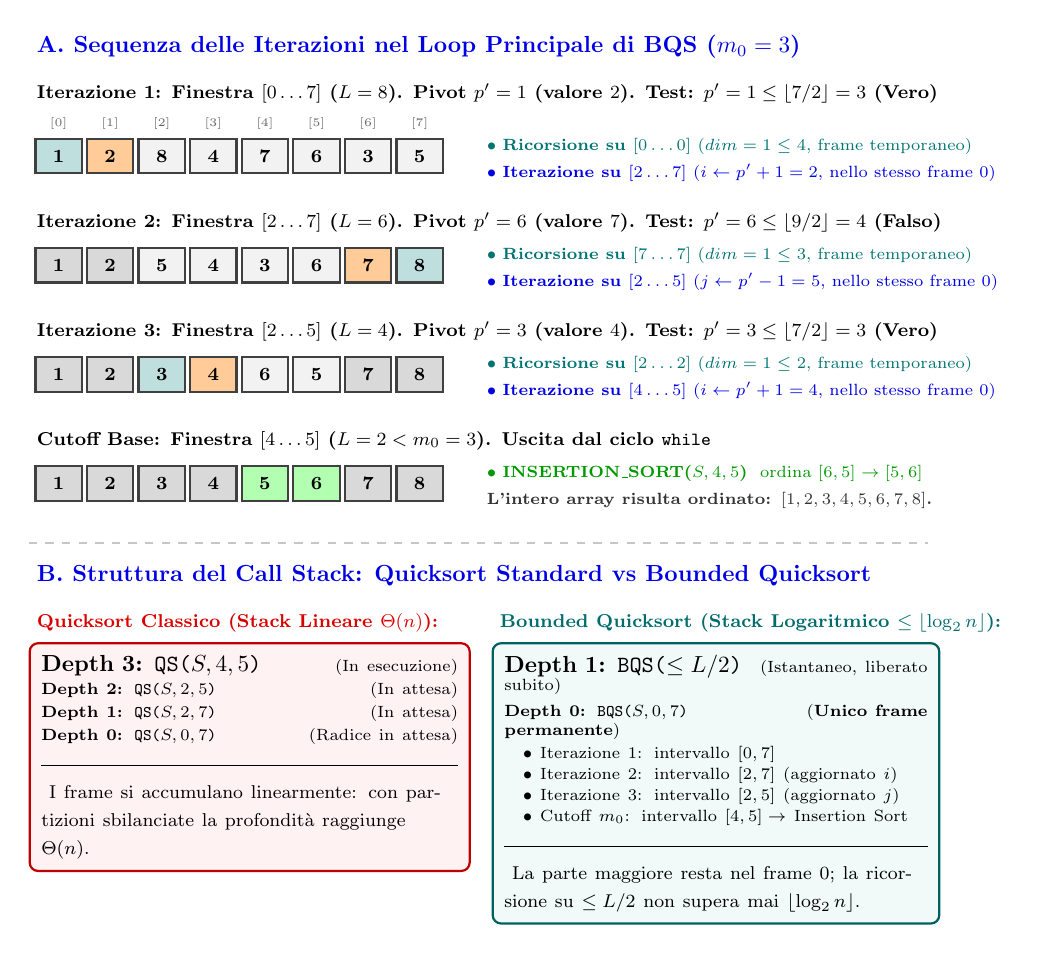
\begin{tikzpicture}[
    scale=0.84,
    every node/.style={transform shape},
    ptr/.style={-{Stealth[scale=1.0]}, very thick, draw=blue!85!black},
    ptrLbl/.style={font=\scriptsize\bfseries, text=blue!90!black},
    cell/.style={rectangle, draw=black!75, thick, minimum width=0.70cm, minimum height=0.52cm, font=\footnotesize\bfseries, align=center},
    frameBox/.style={rectangle, draw=teal!75!black, fill=teal!5, rounded corners=3pt, thick, inner sep=5pt},
    classicBox/.style={rectangle, draw=red!75!black, fill=red!5, rounded corners=3pt, thick, inner sep=5pt}
  ]
    % --- PARTE A: Traccia Esecutiva BQS ---
    \node[anchor=west, font=\normalsize\bfseries, text=blue!90!black] at (0, 8.4) {\textbf{A. Sequenza delle Iterazioni nel Loop Principale di BQS} ($m_0=3$)};

    % Iterazione 1
    \node[anchor=west, font=\footnotesize\bfseries] at (0, 7.7) {Iterazione 1: Finestra $[0 \dots 7]$ ($L=8$). Pivot $p'=1$ (valore $2$). Test: $p'=1 \le \lfloor 7/2 \rfloor = 3$ (Vero)};
    \foreach \val/\col/\idx/\c in {1/teal!25/0/0, 2/orange!40/1/1, 8/gray!10/2/2, 4/gray!10/3/3, 7/gray!10/4/4, 6/gray!10/5/5, 3/gray!10/6/6, 5/gray!10/7/7} {
      \node[cell, fill=\col] at (0.45 + \c*0.78, 6.75) {\val};
      \node[above=0.5pt, font=\tiny\color{black!60}] at (0.45 + \c*0.78, 7.01) {[\idx]};
    }
    \node[anchor=west, font=\scriptsize, text=teal!90!black] at (6.8, 6.9) {$\bullet$ \textbf{Ricorsione su $[0 \dots 0]$} ($\text{dim}=1 \le 4$, frame temporaneo)};
    \node[anchor=west, font=\scriptsize, text=blue!90!black] at (6.8, 6.5) {$\bullet$ \textbf{Iterazione su $[2 \dots 7]$} ($i \leftarrow p'+1=2$, nello stesso frame 0)};

    % Iterazione 2
    \node[anchor=west, font=\footnotesize\bfseries] at (0, 5.75) {Iterazione 2: Finestra $[2 \dots 7]$ ($L=6$). Pivot $p'=6$ (valore $7$). Test: $p'=6 \le \lfloor 9/2 \rfloor = 4$ (Falso)};
    \foreach \val/\col/\c in {1/black!15/0, 2/black!15/1, 5/gray!10/2, 4/gray!10/3, 3/gray!10/4, 6/gray!10/5, 7/orange!40/6, 8/teal!25/7} {
      \node[cell, fill=\col] at (0.45 + \c*0.78, 5.1) {\val};
    }
    \node[anchor=west, font=\scriptsize, text=teal!90!black] at (6.8, 5.25) {$\bullet$ \textbf{Ricorsione su $[7 \dots 7]$} ($\text{dim}=1 \le 3$, frame temporaneo)};
    \node[anchor=west, font=\scriptsize, text=blue!90!black] at (6.8, 4.85) {$\bullet$ \textbf{Iterazione su $[2 \dots 5]$} ($j \leftarrow p'-1=5$, nello stesso frame 0)};

    % Iterazione 3
    \node[anchor=west, font=\footnotesize\bfseries] at (0, 4.1) {Iterazione 3: Finestra $[2 \dots 5]$ ($L=4$). Pivot $p'=3$ (valore $4$). Test: $p'=3 \le \lfloor 7/2 \rfloor = 3$ (Vero)};
    \foreach \val/\col/\c in {1/black!15/0, 2/black!15/1, 3/teal!25/2, 4/orange!40/3, 6/gray!10/4, 5/gray!10/5, 7/black!15/6, 8/black!15/7} {
      \node[cell, fill=\col] at (0.45 + \c*0.78, 3.45) {\val};
    }
    \node[anchor=west, font=\scriptsize, text=teal!90!black] at (6.8, 3.6) {$\bullet$ \textbf{Ricorsione su $[2 \dots 2]$} ($\text{dim}=1 \le 2$, frame temporaneo)};
    \node[anchor=west, font=\scriptsize, text=blue!90!black] at (6.8, 3.2) {$\bullet$ \textbf{Iterazione su $[4 \dots 5]$} ($i \leftarrow p'+1=4$, nello stesso frame 0)};

    % Iterazione 4 (Cutoff)
    \node[anchor=west, font=\footnotesize\bfseries] at (0, 2.45) {Cutoff Base: Finestra $[4 \dots 5]$ ($L=2 < m_0=3$). Uscita dal ciclo \texttt{while}};
    \foreach \val/\col/\c in {1/black!15/0, 2/black!15/1, 3/black!15/2, 4/black!15/3, 5/green!30/4, 6/green!30/5, 7/black!15/6, 8/black!15/7} {
      \node[cell, fill=\col] at (0.45 + \c*0.78, 1.8) {\val};
    }
    \node[anchor=west, font=\scriptsize, text=green!60!black] at (6.8, 1.95) {$\bullet$ \textbf{INSERTION\_SORT($S, 4, 5$)} $\implies$ ordina $[6, 5] \to [5, 6]$};
    \node[anchor=west, font=\scriptsize\bfseries, text=black!80] at (6.8, 1.55) {L'intero array risulta ordinato: $[1, 2, 3, 4, 5, 6, 7, 8]$.};

    % Separatore orizzontale
    \draw[thick, dashed, draw=gray!45] (0, 0.9) -- (13.6, 0.9);

    % --- PARTE B: Confronto Call Stack ---
    \node[anchor=west, font=\normalsize\bfseries, text=blue!90!black] at (0, 0.4) {\textbf{B. Struttura del Call Stack: Quicksort Standard vs Bounded Quicksort}};

    % Stack Classic
    \node[anchor=west, font=\footnotesize\bfseries, text=red!85!black] at (0, -0.3) {Quicksort Classico (Stack Lineare $\Theta(n)$):};
    \node[classicBox, anchor=north west, text width=6.3cm, align=left] at (0, -0.6) {
      \textbf{Depth 3:} \texttt{QS($S, 4, 5$)} \hfill \scriptsize (In esecuzione)\\[2pt]
      \textbf{Depth 2:} \texttt{QS($S, 2, 5$)} \hfill \scriptsize (In attesa)\\[2pt]
      \textbf{Depth 1:} \texttt{QS($S, 2, 7$)} \hfill \scriptsize (In attesa)\\[2pt]
      \textbf{Depth 0:} \texttt{QS($S, 0, 7$)} \hfill \scriptsize (Radice in attesa)\\[3pt]
      \rule{\linewidth}{0.4pt}\\[2pt]
      \footnotesize $\implies$ I frame si accumulano linearmente: con partizioni sbilanciate la profondità raggiunge $\Theta(n)$.
    };

    % Stack BQS
    \node[anchor=west, font=\footnotesize\bfseries, text=teal!85!black] at (7.0, -0.3) {Bounded Quicksort (Stack Logaritmico $\le \lfloor\log_2 n\rfloor$):};
    \node[frameBox, anchor=north west, text width=6.4cm, align=left] at (7.0, -0.6) {
      \textbf{Depth 1:} \texttt{BQS($\le L/2$)} \hfill \scriptsize (Istantaneo, liberato subito)\\[3pt]
      \textbf{Depth 0:} \texttt{BQS($S, 0, 7$)} \hfill \scriptsize (\textbf{Unico frame permanente})\\[2pt]
      \quad $\bullet$ Iterazione 1: intervallo $[0, 7]$\\[1pt]
      \quad $\bullet$ Iterazione 2: intervallo $[2, 7]$ (aggiornato $i$)\\[1pt]
      \quad $\bullet$ Iterazione 3: intervallo $[2, 5]$ (aggiornato $j$)\\[1pt]
      \quad $\bullet$ Cutoff $m_0$: intervallo $[4, 5] \to$ Insertion Sort\\[3pt]
      \rule{\linewidth}{0.4pt}\\[2pt]
      \footnotesize $\implies$ La parte maggiore resta nel frame 0; la ricorsione su $\le L/2$ non supera mai $\lfloor\log_2 n\rfloor$.
    };

  \end{tikzpicture}
  \caption{Traccia dell'esecuzione di Bounded Quicksort (BQS) con soglia $m_0=3$ e confronto della memoria di stack. (\textbf{A}) Ad ogni iterazione, la partizione sbilanciata maggiore viene mantenuta nello stesso stack frame aggiornando $i$ o $j$, mentre solo la partizione dimezzata ($\le L/2$) genera una breve chiamata ricorsiva. (\textbf{B}) Il Quicksort ordinario accumula frame lineari; BQS garantisce uno stack a profondità rigorosamente logaritmica.}
  \label{fig:bqs-trace-and-stack}
\end{figure}

In \autoref{tab:bqs-execution-trace} viene dettagliata la sequenza puntuale delle iterazioni, evidenziando il test sulla partizione minima, l'azione di tail call elimination e la profondità massima istantanea dello stack di esecuzione.

\begin{table}[H]
  \centering
  \noindent\makebox[\textwidth][c]{%
  \footnotesize
  \setlength{\tabcolsep}{4.5pt}
  \begin{tabular}{c c c c l c c}
    \toprule
    \textbf{Passo} & $\boldsymbol{[i, j]}$ & $\boldsymbol{L}$ & \textbf{Test Pivot} & \textbf{Azione (Ricorsione \& Iterazione)} & \textbf{Stato Array} & \textbf{Stack} \\
    \midrule
    Init & $[0, 7]$ & 8 & -- & Frame radice $\text{BQS}(S, 0, 7)$ & $[7, 2, 8, 4, 1, 6, 3, 5]$ & 0 \\
    \addlinespace[3pt]
    1 & $[0, 7]$ & 8 & $p'=1 \le 3$ & 
    \begin{tabular}{@{}ll@{}}
      \textbf{Rec:}  & $[0, 0]$ ($\text{dim} \le 4$, istantanea) \\
      \textbf{Iter:} & $i \leftarrow 2$ su $[2, 7]$ (stesso frame)
    \end{tabular} & $[1 \mid \mathbf{2} \mid 8, 4, 7, 6, 3, 5]$ & 1 \\
    \addlinespace[3pt]
    2 & $[2, 7]$ & 6 & $p'=6 > 4$ & 
    \begin{tabular}{@{}ll@{}}
      \textbf{Rec:}  & $[7, 7]$ ($\text{dim} \le 3$, istantanea) \\
      \textbf{Iter:} & $j \leftarrow 5$ su $[2, 5]$ (stesso frame)
    \end{tabular} & $[1, 2 \mid 5, 4, 3, 6 \mid \mathbf{7} \mid 8]$ & 1 \\
    \addlinespace[3pt]
    3 & $[2, 5]$ & 4 & $p'=3 \le 3$ & 
    \begin{tabular}{@{}ll@{}}
      \textbf{Rec:}  & $[2, 2]$ ($\text{dim} \le 2$, istantanea) \\
      \textbf{Iter:} & $i \leftarrow 4$ su $[4, 5]$ (stesso frame)
    \end{tabular} & $[1, 2 \mid 3 \mid \mathbf{4} \mid 6, 5 \mid 7 \mid 8]$ & 1 \\
    \midrule
    Cutoff & $[4, 5]$ & 2 & $L < m_0$ & 
    \begin{tabular}{@{}ll@{}}
      \textbf{Exit:} & Uscita dal ciclo \texttt{while} \\
      \textbf{Sort:} & Insertion Sort su $[4, 5]$
    \end{tabular} & $[1, 2, 3, 4, \mathbf{5, 6}, 7, 8]$ & 0 \\
    \bottomrule
  \end{tabular}%
  }
  \caption{Traccia dell'esecuzione passo-passo di Bounded Quicksort (BQS) con soglia di cutoff $m_0=3$. In ogni iterazione, la partizione di dimensione minore o uguale a $L/2$ viene risolta con una chiamata ricorsiva limitata, mentre la partizione più grande viene elaborata iterativamente all'interno del frame corrente, mantenendo la profondità dello stack $\le 1$ nell'esempio ($\le \lfloor \log_2 n \rfloor$ nel caso generale).}
  \label{tab:bqs-execution-trace}
\end{table}

\FloatBarrier

\subsection{Analisi Rigorosa dello Spazio Extra \texorpdfstring{$\Theta(\log_2 n)$}{Theta(log n)}}
\label{subsec:bqs-space-analysis}

L'aspetto fondamentale di BQS risiede nella garanzia assoluta sul consumo di memoria di sistema:

\begin{theorem}[Garanzia dello Spazio Ausiliario di Bounded Quicksort]
\label{thm:bqs-space-guarantee}
Per qualsiasi input di $n$ elementi, l'algoritmo Bounded Quicksort alloca uno spazio aggiuntivo sullo stack di sistema rigidamente limitato a:
\begin{equation}
  \text{Spazio Ausiliario} = \Theta(\log_2 n).
\end{equation}
La profondità massima dello stack non eccede $\lfloor \log_2 n \rfloor$ nel caso peggiore assoluto.
\end{theorem}

\begin{proof}
Sia $L$ la lunghezza della finestra corrente dell'array all'ingresso di una chiamata a BQS, definita da $L = j - i + 1$. Quando il pivot viene posizionato nell'indice $p'$, l'algoritmo effettua una diramazione esaminando la dimensione delle due partizioni:
\begin{itemize}
  \item La partizione sinistra ha ampiezza $L_{\text{left}} = (p' - 1) - i + 1 = p' - i$.
  \item La partizione destra ha ampiezza $L_{\text{right}} = j - (p' + 1) + 1 = j - p'$.
\end{itemize}
La condizione del test $p' \le \lfloor \frac{i + j}{2} \rfloor$ impone che:
\begin{equation}
  p' - i \le \frac{j - i}{2} < \frac{L}{2}.
\end{equation}
Pertanto, se la condizione è verificata, la chiamata ricorsiva viene invocata sulla partizione sinistra, la cui dimensione è strettamente limitata da:
\begin{equation}
  L_{\text{ricorsivo}} \le \left\lfloor \frac{L}{2} \right\rfloor.
\end{equation}
Nel caso complementare ($p' > \lfloor \frac{i + j}{2} \rfloor$), la partizione destra soddisfa analogamente $j - p' < \frac{L}{2}$, e la chiamata ricorsiva viene invocata sulla partizione destra, verificando la medesima disequazione.

La partizione rimanente possiede dimensione $L_{\text{iterativo}} \ge \frac{L}{2}$, ma essa \textbf{non genera alcuna chiamata ricorsiva}: l'algoritmo aggiorna semplicemente il puntatore $i \leftarrow p' + 1$ oppure $j \leftarrow p' - 1$ e itera nel corpo del ciclo `while` senza allocare alcun nuovo stack frame.

Ne consegue che la dimensione della sotto-istanza associata a ciascuna chiamata ricorsiva nidificata sullo stack si riduce di almeno un fattore $2$ rispetto al frame genitore:
\begin{equation}
  L^{(k)} \le \frac{n}{2^k},
\end{equation}
dove $k$ rappresenta la profondità corrente dello stack. Il processo di ricorsione può proseguire al massimo fintanto che $L^{(k)} \ge m_0 \ge 1$:
\begin{equation}
  \frac{n}{2^k} \ge 1 \implies 2^k \le n \implies k \le \lfloor \log_2 n \rfloor.
\end{equation}
Poiché ciascun record di attivazione richiede una quantità costante di memoria $\mathcal{O}(1)$, il consumo totale di memoria ausiliaria è rigorosamente limitato a:
\begin{equation}
  \text{Extra Space} = \mathcal{O}(1) \cdot \lfloor \log_2 n \rfloor = \Theta(\log_2 n).
\end{equation}
\end{proof}

\subsection{Ottimizzazione Ibrida con Cutoff a Insertion Sort}
\label{subsec:bqs-cutoff-insertion-sort}

L'introduzione della soglia $m_0 \in [16, 32]$ per il passaggio ad \textit{Insertion Sort} risponde a un criterio fondamentale di \textit{cache locality} ed efficienza esecutiva:

\begin{itemize}
  \item \textbf{Eliminazione dell'overhead ricorsivo:} Quando la dimensione del sottoarray è inferiore a $m_0$, il costo associato alla chiamata di funzione, al partizionamento e alla gestione dei puntatori supera il costo computazionale dei confronti diretti.
  \item \textbf{Efficienza di Insertion Sort sui piccoli blocchi:} \textit{Insertion Sort} possiede un fattore costante di tempo eccezionalmente ridotto: l'algoritmo non necessita di memoria ausiliaria, esegue istruzioni elementari all'interno di un ciclo compatto e beneficia dell'inlining del codice da parte del compilatore.
  \item \textbf{Sfruttamento ottimale della Cache L1:} Un blocco di $16 \div 32$ elementi occupa circa $128 \div 256$ byte (per elementi da 64 bit), risiedendo integralmente all'interno di una o al massimo due linee di cache L1 ($64$ byte per linea). Di conseguenza, tutti i confronti e gli scambi avvengono senza generare alcun cache miss, massimizzando il throughput della CPU.
  \item \textbf{Comportamento su array quasi ordinati:} Poiché le macro-partizioni di Quicksort hanno già collocato gli elementi nelle vicinanze della loro posizione finale, l'esecuzione di Insertion Sort sui blocchi piccoli trova i dati in una configurazione "quasi ordinata", convergendo in un tempo strettamente lineare $\mathcal{O}(n)$ anziché quadratico.
\end{itemize}

In conclusione, Bounded Quicksort rappresenta una perfetta sintesi di rigore teorico e ingegneria algoritmica, garantendo la complessità temporale attesa ottima $\mathcal{O}(n \log_2 n)$, l'immunità da \textit{Stack Overflow} grazie allo spazio extra $\Theta(\log_2 n)$, e la massima velocità empirica su hardware moderno.
